\chapter{Software Simulation}

We develop a software simulation to model the effectiveness of the pinhole mask display. There are multiple motivations for the software simulation. One, a software simulation allows experiment parameters, such as focus distance and physical distance to be adjusted more easily. In addition, a pinhole mask display is costly, and the software simulation is used to fine tune the parameters of the pinhole mask, such as depth and pinhole size. Finally, higher order aberrations are difficult to simulate with ordinary lenses, but Zernike polynomials are easy to incorporate into a software simulation.

\begin{figure}[ht]
  \centering
  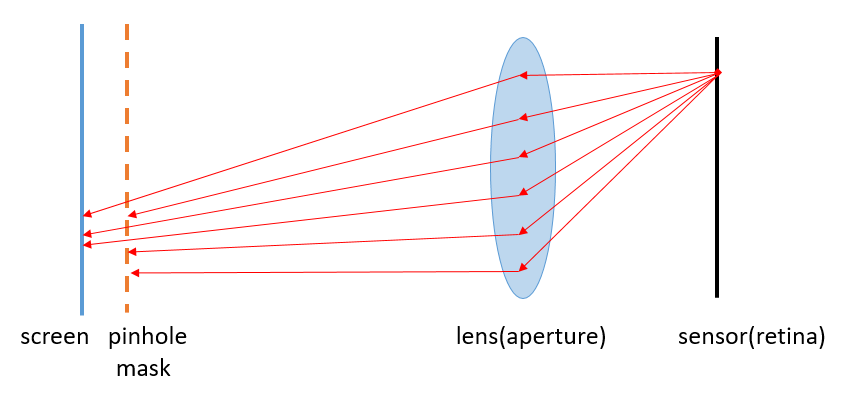
\includegraphics[width=5in]{chapters/chapter6/images/Ray_Simulation.png}
  \caption{Ray Optics Simulation}
  \label{fig:ray_optics}
\end{figure}

One approach we take to simulate the physical experiment is a purely ray optics model. We use a backward ray tracing algorithm, in which light travels from the sensor plane to the display plane. For every pixel on the sensor, the simulation samples multiple points on the aperture (human eye pupil of diameter 6 millimeters). The ray travels straight from the sensor pixel to the aperture point and to the screen. Some of the light rays may get blocked by the pinhole mask or entirely miss the screen. Each screen pixel is composed of a blue, green, and red area, and the color of the ray depends on which position it lands on the screen pixel. Each light ray that reaches the screen contributes to the red, green, or blue intensities of the sensor pixel.

\begin{lstlisting}[frame=single, basicstyle=\footnotesize\ttfamily, caption=Pseudocode For Ray Optics Simulation]
int[][][] sensor = new int[sensor_size][sensor_size][3];
// Iterate over sensor pixels
for (int iy = 0; iy < sensor_size; iy++) {
  for (int ix = 0; ix < sensor_size; ix++) {
    int color[3] = {0, 0, 0};
    int hits = 0;
    // Iterate through random aperture points
    for (int i = 0; i < aperture_sample_time; i++) {
      sensor_pos = (ix, iy);
      aperture_pos = (aperture_samples[2*i], aperture_samples[2*i + 1]);
      type,color = getRayColor(sensor_pos, aperture_pos);
      if (value >= 0) {
        hits++;
	color[type] += value;
      }
    }
  }
  sensor[ix][iy] = color * 3 / hits;
}
\end{lstlisting}

In the physical world, each pixel of light travels straight through free space, through the pupil, and hits a point (rod or cone cell) the retina. Each point on the retina may receive light rays from multiple pixels, so the backward ray tracing algorithm does a good job simulating a human eye. 

Another advantage of this approach is that it is simple and easy to parallelize. With OpenCL, a simulation of an image of size $640\times640$ pixels for roughly $1100$ aperture samples runs in less than one minute. This approach can also take into consideration the quantity of light traveling from the screen to the sensor. If the pinhole size is too small, then too many light rays are blocked by the pinhole mask, and the image on the sensor becomes dim due to the lack of light. To fix this issue, we divided the sum of the light rays by the number of hits. \\
\\
One disadvantage of the ray optics model is that it does not take into account wave properties like diffraction and interference. Even though small pinhole sizes are able to focus light more clearly, they also create larger diffraction effects, which this model does not capture. 